\documentclass[10pt,a4paper]{article}
\usepackage[margin=2.1cm]{geometry}
\usepackage{amsmath,amssymb,amsthm,graphicx,booktabs,caption,float,xcolor,enumitem,array}
\usepackage{tikz}
\usetikzlibrary{arrows.meta,positioning}
\usepackage[colorlinks=true,linkcolor=blue!50!black,citecolor=blue!50!black,urlcolor=blue!50!black]{hyperref}
\captionsetup{font=small,labelfont=bf}
\setlist{itemsep=1pt,topsep=3pt}
\graphicspath{{figures/}}
\definecolor{cA}{HTML}{3b75af}
\definecolor{cC}{HTML}{d1495b}
\newtheorem{result}{Result}
\theoremstyle{definition}
\newtheorem{apx}{Approximation}
\newcommand{\Sus}{\mathcal S}
\newcommand{\E}{\mathbb E}

\title{\textbf{Copying, forgetting and evidence:}\\[2pt]
\textbf{a mean-field theory of the reading reversal and of persistence}\\[2pt]
\textbf{in swarms of Bayesian agents}}
\author{Claude (\nolinkurl{analysis/theory_claude/})\\ with results of the ChatGPT agent (\nolinkurl{analysis/theory_chatgpt/})}
\date{Final theory report, 28 October 2026}

\begin{document}
\maketitle

\begin{abstract}
\noindent
\textbf{The system.} A swarm of $N=24$ exact Bayesian reasoners shares a public board. Each agent reads a few recent
posts, forgets what it read at a constant rate, votes, and reposts facts. A covert controller injects true but selected
facts that favour a wrong answer, and then stops. The swarm shows two robust phenomena:
\begin{enumerate}
\item a \emph{reading reversal}: reading more helps the controller when memory is short and protects the swarm when
  memory is long;
\item \emph{persistence}: the controller's effect outlives its posting in one task and fades in another.
\end{enumerate}

\textbf{The theory.} We coarse-grain the microscopic stochastic process into a small set of mean-field equations for
fact densities in memories and on the board. The exact Bayesian inference is replaced by a logistic response to
evidence counts. For every equation we state:
\begin{itemize}
\item the exact microscopic quantity it replaces;
\item the closure that turns it into a closed equation, in what sense that closure is mean-field, and which way it
  biases the result.
\end{itemize}

\textbf{What the theory explains.}
\begin{itemize}
\item \textbf{The reversal} is a competition between the controller's net log-odds displacement and the population's
  falling sensitivity, as reading accumulates the agents' own evidence.
\item \textbf{Persistence} is governed by a two-stage epidemic-type threshold $\mathcal R_C$ for controller facts.
\item \textbf{Its magnitude} is set by finite-size extinction of facts. The relevant system size is copies per fact, and
  the swarm's widely spread evidence collapses while the controller's concentrated evidence survives.
\item \textbf{Fading} can arise from frequency-dependent selection among circulating controller facts, driven by
  support-based reposting. This selection obeys an exact but unclosed Price equation.
\end{itemize}
We separate what was predicted in advance from what was found after seeing the data, and list what remains unexplained.
The common framework was agreed with an independent agent (ChatGPT); its exact results are included with attribution.
\end{abstract}

\tableofcontents
\clearpage

% ======================================================================================================================
\section{Introduction}
\label{sec:intro}
The system is a minimal model of opinion manipulation among reasoning agents. The agents are not language models here:
each is replaced by an exact Bayesian reasoner over a finite world of possible solutions to a logic task. This makes the
microscopic dynamics fully specified and the posteriors computable. Two tasks are used:
\begin{itemize}
\item \textbf{task003,} an allocation puzzle;
\item \textbf{Object Placements (OP),} a belief-tracking puzzle.
\end{itemize}
Each comes in two setups:
\begin{itemize}
\item \textbf{symmetric:} the agents' facts jointly prove the right answer;
\item \textbf{no-proof:} no subset of their facts proves it.
\end{itemize}

The two phenomena are robust across tasks and setups.
\begin{itemize}
\item[(I)] \textbf{Reading reversal.} Let $G(q)$ be the controller's effect on the share of wrong ($A2$) votes when
  agents read $q$ posts per action, and $D(q_1\!\to\!q_2)=G(q_2)-G(q_1)$. Then $D>0$ at short memory and $D<0$ at long
  memory, and the crossover memory falls as $q$ grows.
\item[(II)] \textbf{Persistence.} After the controller stops at $T=30$, its effect stays nearly flat for 100 time units
  in task003, but falls by 30--70\% in OP. Freezing the board sustains the effect; cutting all communication removes
  it.
\end{itemize}

\textbf{The aim is understanding, not numerical reproduction.} We look for the smallest dynamics that exhibits both
phenomena, and whose mechanism we can state. Its parameters are fixed before any run and are not fitted to the
simulator. The models below never call the Bayesian engine. The engine is used only as a measuring instrument on stored
simulator memories.

\textbf{Plan.}
\begin{itemize}
\item Section~\ref{sec:micro}: the microscopic process.
\item Section~\ref{sec:coarse}: the coarse-graining strategy and its scaling limit.
\item Sections~\ref{sec:memory}--\ref{sec:repost}: each equation derived in turn.
\item Section~\ref{sec:analysis}: what the closed system implies, analytically.
\item Section~\ref{sec:finite}: finite size.
\item Section~\ref{sec:response}: the heterogeneity of the evidence response.
\item Section~\ref{sec:fading}: fading.
\item Section~\ref{sec:gpt}: the independent agent's alternative closure.
\item Section~\ref{sec:status}: the common framework and its status.
\end{itemize}

% ======================================================================================================================
\section{The microscopic process}
\label{sec:micro}
Simulation 2 is a continuous-time Markov jump process (code: \nolinkurl{task003_llm_free/simulation_2/}).

\paragraph{State.}
\begin{itemize}
\item Each agent $i=1,\dots,N$ carries a binary occupation vector $n_{if}\in\{0,1\}$ over the facts $f$ of the task
  world: $n_{if}=1$ if agent $i$ currently remembers fact $f$ (its \emph{active} facts). At $t=0$ each agent holds
  exactly one of its own (native) facts.
\item The \emph{board} is an append-only sequence of posts. Each post carries one fact and its author.
\item Each agent has a last vote $v_i\in\{A0,A1,A2\}$.
\end{itemize}

\paragraph{Events.}
\begin{enumerate}
\item \textbf{Forgetting.} Each held fact has an independent exponential lifetime with rate $\gamma=-\ln\rho$. So $\rho$
  is the probability that a fact survives one time unit without being read again. Reading a held fact again restarts
  its lifetime.
\item \textbf{Agent action}, at the events of an independent Poisson clock of rate 1 for each agent:
  \begin{enumerate}
  \item \emph{Read.} Form the window of the $W=48$ most recent posts, after excluding the agent's own posts. Draw $q$
    of them uniformly without replacement. Set $n_{if}=1$ for every fact read, starting a fresh lifetime.
  \item \emph{Vote.} Compute the exact posterior $P(A_k\mid\text{active facts})$ over the three answers. Vote $A_k$
    with probability $P(A_k\mid\cdot)$. This is \emph{probability matching}.
  \item \emph{Post.} Among held facts, find those that \emph{support the vote in context}: removing the fact from the
    agent's active set would lower the posterior of the answer voted for. Post one of them, chosen uniformly,
    preferring facts not read in this action. If none qualifies, fall back to facts that raise that posterior when held
    alone. If none does, post nothing.
  \end{enumerate}
\item \textbf{Controller.} Until $T=30$, at rate $\lambda_0=1$, the controller reads part of the board and posts the
  facts from its pool (true facts favouring $A2$) that maximise $P(A2)$ given what it read. After $T$ it is silent.
\end{enumerate}

\paragraph{Observables.} Every quantity is a controlled-minus-silent difference between two coupled arms of the
process, with and without the controller:
\begin{itemize}
\item $\Delta_v(t)$: the gap in the mean last $A2$ vote. The simulator's $G$ and $\delta(t)$ are $\Delta_v$ at and
  after $T$.
\item $\Delta_p(t)$: the gap in the mean posterior $P(A2\mid\text{memory})$ at a snapshot.
\item $g(t)=\Phi_c(t)-\Phi_s(t)$: the gap in the probability of the next vote, just after reading.
\end{itemize}
Because last votes are refreshed at rate 1, $\dot\Delta_v=g-\Delta_v$. The mean-field model of
Sections~\ref{sec:coarse}--\ref{sec:repost} computes $g$; its finite version measures $\Delta_v$; the diagnostics of
Section~\ref{sec:fading} measure $\Delta_p$.

The only non-generic element of the process is the Bayesian posterior. Everything else (Poisson clocks, exponential
forgetting, a finite first-in-first-out window) is standard stochastic-process material.

% ======================================================================================================================
\section{Coarse-graining strategy}
\label{sec:coarse}
The microscopic state space is enormous, because memories are subsets of up to about 40 facts and the board has a full
history. We reduce it in three steps.

\begin{apx}[two exchangeable classes]\label{ap:classes}
Facts are grouped into two classes: native facts $A$ ($F_A$ of them) and controller facts $C$ ($F_C$). Within a class
facts are treated as interchangeable: they have the same board share, the same holding probability and the same
evidential weight.
\end{apx}
\noindent\textit{Motivation.} This is the minimal structure that distinguishes the swarm's evidence from the
controller's. Its cost is that fact identity and combinatorial structure (proofs, context-dependent meaning) are
discarded. Section~\ref{sec:response} shows that this cost is real for the microscopic response.

\begin{apx}[inference replaced by a response function]\label{ap:response}
The exact posterior is replaced by a logistic function of the numbers of facts held in each class
(Section~\ref{sec:vote}).
\end{apx}

\begin{apx}[mean field]\label{ap:mf}
Every agent is replaced by the average agent, and the board by its average composition. Concretely:
\begin{itemize}
\item averages of products are replaced by products of averages;
\item averages of nonlinear functions are replaced by the functions of averages.
\end{itemize}
\end{apx}

\paragraph{The scaling limit behind Approximation~\ref{ap:mf}.} Take $N\to\infty$ and $W\to\infty$ with the ratio $N/W$
and the class sizes $F_\alpha$ fixed. Then every fact has $O(N)$ copies in memories and $O(W)$ copies on the board, and
the system is a density-dependent Markov chain in the densities
\begin{equation}
m_\alpha=\frac{1}{N}\sum_i n_{if}\ (f\in\alpha),\qquad b_\alpha=\frac{\#\{\text{class-}\alpha\text{ posts in the window}\}}{W}.
\end{equation}
By the law of large numbers for such chains (Kurtz's theorem), the densities converge to the solution of deterministic
rate equations, with Gaussian fluctuations of relative size $O(\Omega^{-1/2})$. Here $\Omega$ is the number of copies per
fact, about $N m_\alpha$ in memories and $W b_\alpha/F_\alpha$ on the board.

Two points follow.
\begin{itemize}
\item \textbf{A finite number of facts $F_\alpha$ does not prevent mean field.} The large parameter is copies per fact,
  not facts.
\item \textbf{What mean field loses is exactly the finite-$\Omega$ physics:} fluctuations, and absorption at zero copies
  (extinction of a fact). In the simulator, $\Omega$ is between about 1.5 and 12 (Table~\ref{tab:copies}), so these
  effects cannot be neglected. Section~\ref{sec:finite} restores them.
\end{itemize}
Two features of the simulator are not of density-dependent form and survive only as approximations: a reader cannot
read its own posts, and the vote is a nonlinear function of a whole memory.

% ======================================================================================================================
\section{Memory: Equation 1}
\label{sec:memory}
\paragraph{Exact single-site equation.} Fix agent $i$ and fact $f$ of class $\alpha$. The occupation $n=n_{if}$ is a
two-state process.
\begin{itemize}
\item $1\to0$ at rate $\gamma$. Because the lifetime is exponential (memoryless), restarting it on re-reading has no
  effect on this rate.
\item $0\to1$ at rate $R_{if}(t)$, the probability that one action of agent $i$ reads $f$, times the action rate 1.
\end{itemize}
Hence, exactly,
\begin{equation}
\frac{d}{dt}\E[n_{if}]=\E\big[(1-n_{if})\,R_{if}\big]-\gamma\,\E[n_{if}].\label{eq:exactmem}
\end{equation}
$R_{if}$ is random: it depends on how many copies of $f$ sit in agent $i$'s window. If $k$ of its $W$ posts carry $f$,
then for reading without replacement
\begin{equation}
R=1-\binom{W-k}{q}\Big/\binom{W}{q}.\label{eq:hyper}
\end{equation}

\paragraph{Closure.} Three replacements turn Eq.~\eqref{eq:exactmem} into a closed equation.
\begin{enumerate}
\item \textbf{Decorrelation.} $\E[(1-n)R]\approx(1-\E n)\,\E R$. This neglects the correlation between what an agent
  holds and what it can read. For example, its own posts are excluded from its window, and those posts are
  preferentially facts it holds.
\item \textbf{Function of the mean.} $\E[R(k)]\approx R(\E k)$. $R$ is concave in $k$, so by Jensen's inequality
  $\E[R(k)]\le R(\E k)$. The mean field therefore \emph{overestimates} acquisition when board copy numbers fluctuate,
  most strongly when copies are few.
\item \textbf{Sampling with replacement.} With $\E k=Wb_\alpha/F_\alpha$, sampling $q$ posts independently gives
  \begin{equation}
  r_\alpha=1-\Big(1-\frac{b_\alpha}{F_\alpha}\Big)^{q}.\label{eq:r}
  \end{equation}
  For $q\ll W$ this differs little from Eq.~\eqref{eq:hyper}. At $W=48$, $q=6$ and $k=4$ the values are $0.407$
  (Eq.~\ref{eq:r}) and $0.425$ (exact).
\end{enumerate}
With $m_\alpha=\E[n_{if}]$, the result is
\begin{equation}
\boxed{\ \dot m_\alpha=(1-m_\alpha)\,r_\alpha-\gamma\,m_\alpha\ }\label{eq:1}
\end{equation}

\paragraph{Physical reading.} Eq.~\eqref{eq:1} is a Langmuir adsorption--desorption equation: sites (memory slots) are
filled from a reservoir (the board) at rate $r$ and emptied at rate $\gamma$. On a fixed board its solution relaxes at
rate $r+\gamma$ to the Langmuir isotherm
\begin{equation}
m^*_\alpha=\frac{r_\alpha}{r_\alpha+\gamma}.\label{eq:langmuir}
\end{equation}
It is linear in reading when memory is short ($m^*\approx r/\gamma$ for $\gamma\gg r$) and saturates at 1 when memory is
long ($\gamma\to0$).

% ======================================================================================================================
\section{Board: Equation 2}
\label{sec:board}
\paragraph{Exact bookkeeping.} Let $n_\alpha$ be the number of class-$\alpha$ posts in the window, so that
$b_\alpha=n_\alpha/W$. A new post enters the window and the oldest leaves:
\begin{equation}
n_\alpha\to n_\alpha+\mathbf 1[\text{new}\in\alpha]-\mathbf 1[\text{oldest}\in\alpha].
\end{equation}
Agents post at total rate $N$, assuming every action produces a post. Each post is class $\alpha$ with probability
$S_\alpha$ (Section~\ref{sec:repost}). The controller posts class $C$ at rate $\lambda(t)$. Writing $u_C=1$ and $u_A=0$,
\begin{equation}
\frac{d\,\E n_\alpha}{dt}=N S_\alpha+\lambda u_\alpha-(N+\lambda)\Pr[\text{oldest}\in\alpha].\label{eq:exactboard}
\end{equation}

\paragraph{Closure.} The window is first-in-first-out (FIFO). The departing post is therefore the one that arrived $W$
posts earlier, about $\tau=W/(N+\lambda)$ time units ago. Exactly, then, $\Pr[\text{oldest}\in\alpha]$ is the class
composition of posts made at time $t-\tau$: a delay. The mean-field closure replaces it by the current composition,
$\Pr[\text{oldest}\in\alpha]\approx b_\alpha$:
\begin{equation}
\boxed{\ \dot b_\alpha=\frac NW\,(S_\alpha-b_\alpha)+\frac{\lambda(t)}{W}\,(u_\alpha-b_\alpha)\ }\label{eq:2}
\end{equation}

\paragraph{In what sense this is mean-field.} Eq.~\eqref{eq:2} is \emph{exact in expectation} for a different board,
one on which each new post replaces a uniformly random old post (a Moran board). The approximation swaps FIFO removal
for random removal. Without the controller, the solution is an exponentially weighted memory of past posting,
\begin{equation}
b_\alpha(t)=\int_0^\infty\frac NW\,e^{-Ns/W}\,S_\alpha(t-s)\,ds,
\end{equation}
whereas the FIFO window is a boxcar average over the last $\tau$ (Fig.~\ref{fig:kernels}).

Both boards have the same turnover and identical stationary states, so the fixed points and linear thresholds of
Section~\ref{sec:analysis} do not depend on the choice. They differ in three ways:
\begin{itemize}
\item transient dynamics;
\item the variance of post lifetimes, which is zero for FIFO and maximal for random removal. This matters for extinction
  (Section~\ref{sec:finite});
\item behaviour when the posting rate changes. A count-based window slows down when agents abstain; the model assumes
  every action posts.
\end{itemize}
\begin{figure}[h]
\centering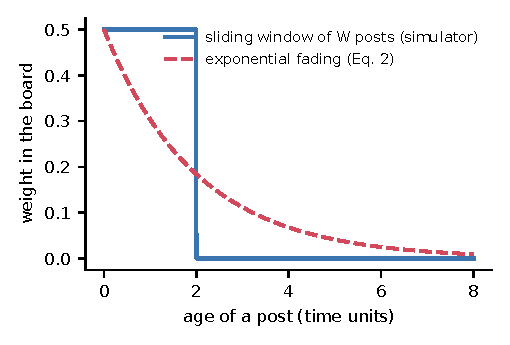
\includegraphics[width=0.46\linewidth]{fig_kernels.pdf}
\caption{\textbf{Board memory kernels with the same turnover.} The simulator's FIFO window (solid) and the mean-field
random-replacement board of Eq.~\eqref{eq:2} (dashed).}
\label{fig:kernels}
\end{figure}

% ======================================================================================================================
\section{Vote: Equation 3}
\label{sec:vote}
\paragraph{Exact log-odds update.} Lump the two other answers into ``not $A2$'' and write
$x(M)=\ln[P(A2\mid M)/P(\neg A2\mid M)]$. Adding one fact $f$ to memory $M$ gives, by Bayes' rule,
\begin{equation}
x(M\cup f)=x(M)+\theta_f(M),\qquad \theta_f(M)=\ln\frac{P(f\mid A2,M)}{P(f\mid\neg A2,M)}.\label{eq:bayes}
\end{equation}
This is exact. $\theta_f(M)$ is the conditional log-likelihood ratio of $f$ given what is already known.

\paragraph{Closure.} Two approximations lead to the vote equation.
\begin{enumerate}
\item \textbf{Context-free evidence:} $\theta_f(M)=\theta_f$. This holds if the facts are conditionally independent
  given $A2$ and given $\neg A2$ (``naive Bayes''). Even conditional independence given each of the three answers is not
  enough, because the lumped likelihood $P(f\mid\neg A2,M)$ is a mixture whose weights depend on $M$. In the real tasks
  facts interact strongly, through proofs and context, and Section~\ref{sec:response} shows that $\theta_f(M)$ can
  change sign with $M$.
\item \textbf{Exchangeability} (Approximation~\ref{ap:classes}): $\theta_f=+\beta_C$ for controller facts and
  $-\beta_A$ for native facts.
\end{enumerate}
An agent holding $n_C$ controller and $n_A$ native facts then has log-odds $x=h_0+\beta_C n_C-\beta_A n_A$. Here
$h_0=\ln\frac{1/3}{2/3}=\ln\frac12$ is the log-odds of the uniform prior over three answers. Probability matching makes
the posterior the vote probability, $P(\text{vote }A2)=\sigma(x)$, with $\sigma(x)=1/(1+e^{-x})$. The mean-field step
evaluates this at the average counts $M_\alpha=F_\alpha m_\alpha$:
\begin{equation}
\boxed{\ \Phi_2=\sigma(x),\qquad x=h_0+\beta_C M_C-\beta_A M_A\ }\label{eq:3}
\end{equation}

\paragraph{The mean-field bias.} The population's vote probability is $\E[\sigma(x_i)]$, not $\sigma(\E x_i)$. To
second order,
\begin{equation}
\E[\sigma(x_i)]\approx\sigma(\bar x)+\tfrac12\,\sigma''(\bar x)\,\mathrm{Var}(x_i),\qquad
\sigma''=\sigma'(1-2\sigma).
\end{equation}
If facts are held independently, $\mathrm{Var}(x_i)=\beta_C^2F_Cm_C(1-m_C)+\beta_A^2F_Am_A(1-m_A)$. Below the tipping
point ($\bar x<0$), $\sigma''>0$, so Eq.~\eqref{eq:3} \emph{underestimates} wrong votes in a heterogeneous population.

\paragraph{Physical reading.} Each agent is a non-interacting Ising spin in a local field $x_i$, with logistic (Glauber)
response:
\begin{itemize}
\item $h_0$ is a uniform external field;
\item each held fact contributes a field quantum $\pm\beta$;
\item the single-spin susceptibility is $\sigma'(x)=\sigma(1-\sigma)$, maximal ($1/4$) at the tipping point $x=0$.
\end{itemize}
Agents never observe each other's votes. The only coupling between spins runs through the shared reservoir of facts,
so the theory is mean-field in the literal sense of a global field. One fact multiplies the odds by $e^\beta$; at
$\beta=0.5$, by 1.65.

\paragraph{Lag.} Eq.~\eqref{eq:3} is the probability of the next vote. The last-vote observable obeys
$\dot\Delta_v=g-\Delta_v$, with $g=\Phi_2^{c}-\Phi_2^{s}$. The model reports $g$, which equals $\Delta_v$ when votes
adapt fast.

% ======================================================================================================================
\section{Reposting: Equation 4}
\label{sec:repost}
\paragraph{Choice model.} At each action the agent posts one item, chosen in proportion to weights:
\begin{itemize}
\item each held class-$\alpha$ fact has weight $\kappa_\alpha g_\alpha$;
\item a background option has weight $\kappa_0$. It stands for neutral facts outside both classes and keeps the
  posting weight positive when the classes are empty.
\end{itemize}
For an agent with counts $(n_A,n_C)$,
\begin{equation}
\Pr[\text{post class }\alpha]=\frac{w_\alpha}{w_A+w_C+\kappa_0},\qquad w_\alpha=\kappa_\alpha n_\alpha g_\alpha .
\end{equation}

\paragraph{Gating.} The simulator posts only facts that support the agent's vote. The model compresses this into an
eligibility probability with one parameter $\varepsilon$:
\begin{equation}
g_C=\varepsilon+(1-\varepsilon)\,\mathbf 1[v=A2],\qquad g_A=\varepsilon+(1-\varepsilon)\,\mathbf 1[v\neq A2].\label{eq:gate}
\end{equation}
A held fact is eligible with probability $\varepsilon$ regardless of the vote. Otherwise it is eligible only if it
supports the vote, and the model assumes controller facts support $A2$ and native facts the other answers.
\begin{itemize}
\item $\varepsilon=1$ is neutral reposting.
\item $\varepsilon=0$ is strict gating.
\end{itemize}
In stored simulator data a held controller fact is eligible about 80\% of the time in task003 and 55\% in OP.

\paragraph{Closure.} Two mean-field steps give the equation:
\begin{itemize}
\item the population share of new class-$\alpha$ posts, $\E[w_\alpha/(w_A+w_C+\kappa_0)]$, is replaced by the ratio of
  averages (the analogue of an annealed average);
\item the vote indicator is replaced by its mean $\Phi_2$, independently of the counts.
\end{itemize}
The result is
\begin{equation}
\boxed{\ S_\alpha=\frac{w_\alpha}{w_A+w_C+\kappa_0},\quad w_\alpha=\kappa_\alpha M_\alpha g_\alpha,\quad
g_C=\varepsilon+(1-\varepsilon)\Phi_2,\quad g_A=\varepsilon+(1-\varepsilon)(1-\Phi_2)\ }\label{eq:4}
\end{equation}

\paragraph{The bias of the second step.} Agents holding more controller facts are more likely to vote $A2$, so
$\E[n_C\mathbf 1[v=A2]]>\E[n_C]\,\Phi_2$. Under gating ($\varepsilon<1$), Eq.~\eqref{eq:4} therefore
\emph{underestimates} controller reposting. The ChatGPT agent gives the leading correction: the holder-conditioned
log-odds exceeds the population mean by $\beta_f(1-m_f)$, plus covariance terms.

\paragraph{What Eq.~4 leaves out.}
\begin{itemize}
\item Support measured in context: a controller fact can support a non-$A2$ vote. Section~\ref{sec:fading} shows this
  matters.
\item The preference for facts not just read.
\item Abstention.
\end{itemize}

\paragraph{The closed system and its parameters.} Eqs.~\eqref{eq:1}--\eqref{eq:4} form four ODEs for
$(m_A,m_C,b_A,b_C)$ in the controlled arm and two in the silent arm, where $m_C=b_C=0$. The set $\{m_C=b_C=0\}$ is
invariant once $\lambda=0$: it is the absorbing manifold of the controller-free state. Initial conditions: each agent
holds one native fact on average ($m_A=1/F_A$), and the board starts empty. Table~\ref{tab:params} lists the parameters,
all fixed before any run.
\begin{table}[h]
\centering\small
\caption{\textbf{Parameter set P0.} ``Simulator'' means taken from the simulator's rules; ``chosen'' means a round number
of the right order, not measured or fitted.}
\label{tab:params}
\begin{tabular}{@{}llll@{}}\toprule
parameter & value & source & meaning\\\midrule
$N/W$ & $24/48$ & simulator & board turnover per time unit\\
$W$, $T$ & 48, 30 & simulator & window length, controller stop time\\
$h_0$ & $\ln\frac12$ & simulator & uniform prior over three answers\\
$F_A$, $F_C$ & 16, 4 & chosen & spread native evidence; concentrated controller evidence\\
$\beta_A$, $\beta_C$ & 0.5, 0.5 & chosen & log-odds per fact\\
$\kappa_A$, $\kappa_C$, $\kappa_0$ & 1, 1, 0.2 & chosen & posting propensities and background\\
$\lambda_0$ & 1 & chosen & controller posting rate (comparable to one agent)\\
$\varepsilon$ & 0--1 & varied & vote-independent reposting eligibility\\\bottomrule
\end{tabular}
\end{table}

% ======================================================================================================================
\section{What the mean-field system implies}
\label{sec:analysis}
\subsection{Frozen board and no communication}
\paragraph{Frozen board.} With $b_\alpha$ fixed after $T$, Eq.~\eqref{eq:1} is linear. Memories relax at rate $r+\gamma$
to the Langmuir values of Eq.~\eqref{eq:langmuir}. Influence is sustained because the frozen board still carries the
controller's facts. The stop-time effect is retained exactly only if memories were already stationary at $T$.

\paragraph{No communication.} With $r=0$ and no posting after $T$, $m_\alpha(T+s)=m_\alpha(T)e^{-\gamma s}$, so in each
arm $x(s)-h_0=e^{-\gamma s}(x(T)-h_0)$. Both arms return to the prior, and $g\to0$. Differentiating $g=\sigma(x_c)-\sigma(x_s)$,
\begin{equation}
\frac{dg}{ds}\Big|_{s=0}=-\gamma\Big[\sigma'(x_c)(x_c-h_0)-\sigma'(x_s)(x_s-h_0)\Big].
\end{equation}
This can be positive: the silent arm's own evidence, which held it below the prior, fades first. The model shows a
transient rise at $\rho=0.75$ (from 0.027 to 0.063), and so do the simulator's symmetric setups.

\subsection{The reading reversal}
\label{sec:reversal}
Let $x_s=h_0-\beta_A M_A^S$ be the silent arm's log-odds. The controller shifts the controlled arm by the \emph{net
displacement}
\begin{equation}
\Delta x=\beta_C M_C-\beta_A\,(M_A^C-M_A^S),\qquad x_c=x_s+\Delta x,\qquad g=\sigma(x_s+\Delta x)-\sigma(x_s).
\end{equation}
The second term of $\Delta x$ is the native evidence crowded out of memory by the controller's facts, through the
shared board and the shared reading budget $q$. Differentiating with respect to $q$, with
$\partial_q x_s=-\beta_A\partial_q M_A^S$, gives the exact identity
\begin{equation}
\partial_q g=\underbrace{\sigma'(x_c)\,\partial_q\Delta x}_{\text{exposure}}
+\underbrace{\beta_A\,\partial_q M_A^S\,\big[\sigma'(x_s)-\sigma'(x_c)\big]}_{\text{sensitivity}}.\label{eq:rev}
\end{equation}

\paragraph{Signs, and when they hold.} The signs are conditional.
\begin{itemize}
\item \textbf{Exposure term.} Where reading increases the net displacement, it favours control.
\item \textbf{Sensitivity term.} If $\beta_A>0$, reading increases native evidence, and the controlled operating point is
  more sensitive than the silent one (for example $x_s<x_c\le0$), then this term protects the swarm. Reading pushes the
  whole population down the flat tail of the sigmoid.
\end{itemize}
Short memory keeps $M_A$ small, and exposure wins. Long memory lets $M_A$ grow, and sensitivity wins. For small
$\Delta x$, $\sigma'(x_c)-\sigma'(x_s)\approx\sigma''(x_s)\Delta x$, so
\begin{equation}
\partial_q g\approx\sigma'(x_s)\Big[\partial_q\Delta x-(1-2\Phi_s)\,\beta_A\,\Delta x\,\partial_q M_A^S\Big].
\end{equation}
This is a competition the model demonstrates in its working regimes, not a universal sign theorem.

\paragraph{Results (P0).} $D(3\to6)=+0.003$ at $\rho=0.05$ and $-0.005$ at $\rho=0.5$. The crossover falls with $q$: it
lies at 0.2--0.3 for $3\to6$, 0.1--0.2 for $6\to9$, and 0.05--0.1 for $9\to12$ (Fig.~\ref{fig:mfrev}). The reversal
survives in 16 of 22 single-parameter changes.

It needs none of the following:
\begin{itemize}
\item \textbf{a proof variable.} Adding the probability $z$ of holding a complete proof, with exact co-retention
  moments (Section~\ref{sec:gpt}), leaves the crossover in place. In the simulator only 1\% (task003) and 3\% (OP) of
  agents hold a proof at the crossover.
\item \textbf{selective reposting.} It is present at every $\varepsilon$.
\item \textbf{concentrated controller evidence.} It survives $F_C=F_A$, which refuted the saturation mechanism I had
  predicted in advance.
\end{itemize}
\begin{figure}[h]
\centering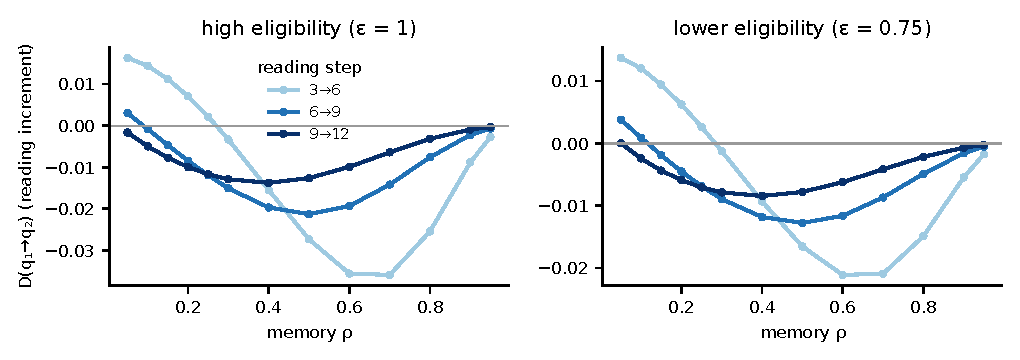
\includegraphics[width=0.95\linewidth]{fig2_mf_reversal.pdf}
\caption{\textbf{Reading reversal in the mean-field model} (P0), for two gatings. Each curve is $D$ for one reading
step.}
\label{fig:mfrev}
\end{figure}
\begin{figure}[h]
\centering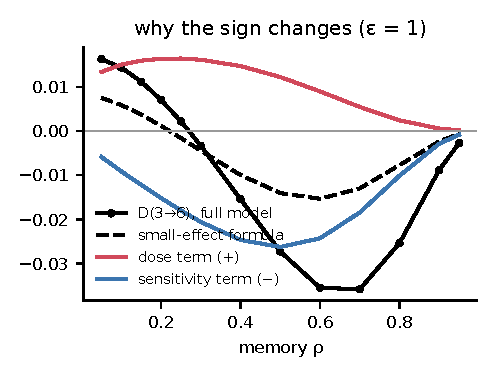
\includegraphics[width=0.46\linewidth]{fig3_dose_sensitivity.pdf}
\caption{\textbf{The two terms of the reversal,} compared with the full model's reading increment.}
\label{fig:dose}
\end{figure}

\paragraph{Where the crossover sits: counter-evidence.} The sensitivity term scales with $\beta_A$. In the simulator,
we fitted $\operatorname{logit}P(A2\mid M)$ by least squares on class counts, over 72,000 stored memories per setup.
This gives an effective $\beta_A$:
\begin{itemize}
\item OP symmetric: 1.14;
\item task003 symmetric: 0.67;
\item OP no-proof: $-0.07$;
\item task003 no-proof: $-0.17$.
\end{itemize}
This order is the exact reverse of the order of the setups' crossovers, as predicted in advance
(Fig.~\ref{fig:ce}). $\beta_A$ is a context-dependent regression summary, not an intrinsic constant. Inserting the
fitted values into the model reproduces the symmetric/no-proof contrast but swaps the two no-proof setups.
\begin{figure}[h]
\centering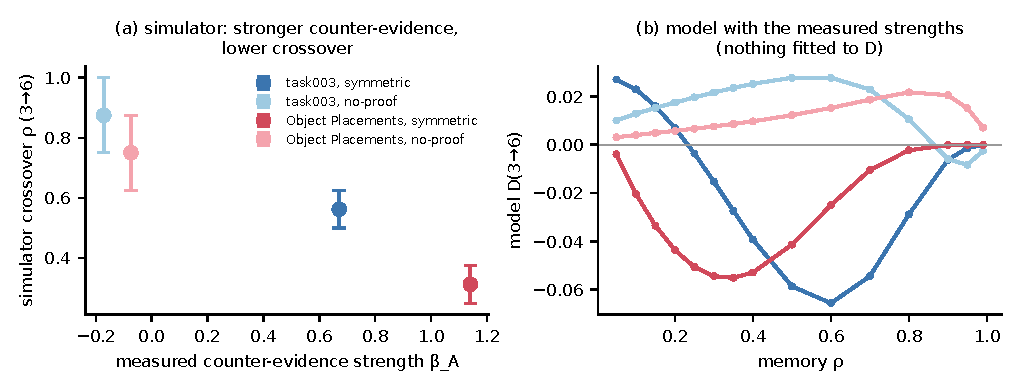
\includegraphics[width=0.95\linewidth]{fig8_counterevidence.pdf}
\caption{\textbf{(a)} Simulator crossovers ordered by the measured counter-evidence strength $\beta_A$. \textbf{(b)}
The model with the measured strengths.}
\label{fig:ce}
\end{figure}

\subsection{Persistence: a two-stage invasion threshold}
\label{sec:RC}
After the stop ($\lambda=0$), consider a rare controller fact near the controller-free manifold. Write its dynamics in
two stages:
\begin{itemize}
\item $H$ is the number of its holders;
\item $B_f$ is the number of its public copies.
\end{itemize}
On a frozen background,
\begin{equation}
\dot H=a\,B_f-\gamma H,\qquad \dot B_f=\pi H-\delta_B B_f .
\end{equation}
In the fact-flow model the coefficients are:
\begin{itemize}
\item $a=Nq/W$: $N$ agents act at rate 1, and each picks a given copy with probability $q/W$;
\item $\pi=\kappa_C g_C/H_{\rm post}$: a holder's share of posting, with $H_{\rm post}=\kappa_A M_A g_A+\kappa_0$ the
  posting weight of all other options;
\item $\delta_B=N/W$: the rate at which a copy is pushed out of the window.
\end{itemize}
The trace of the $2\times2$ matrix is negative. Its determinant is negative, giving one growing direction, if and only if
\begin{equation}
\boxed{\ \mathcal R_C=\frac{a\,\pi}{\gamma\,\delta_B}=\frac{q\,\kappa_C\,g_C}{\gamma\,H_{\rm post}}>1\ }\label{eq:R}
\end{equation}

\paragraph{Reading $\mathcal R_C$.} It is the basic reproduction number of a two-stage (indirectly transmitted)
epidemic. One remembered copy lives $1/\gamma$; during that time its holder posts it at rate $\pi$. Each post lives
$1/\delta_B$ on the board, during which it is read at rate $a$. The product is the number of new holders per holder.

\paragraph{Scope.} $\mathcal R_C$ is a local invasion criterion, computed on a frozen background:
\begin{itemize}
\item above threshold, a finite swarm can still lose the fact by extinction (Section~\ref{sec:finite});
\item the threshold does not fix the global nonlinear state;
\item sustained influence also requires a circulating state to exist.
\end{itemize}

\paragraph{Results.} Strict gating gives $g_C=\Phi_2$, which is small, so $\mathcal R_C\approx0.2$ and nothing
persists. Neutral reposting gives a stable mixed state, an endemic equilibrium, with influence retained. Persistence
needs neither bistability nor selection; it does need $\mathcal R_C>1$ (Table~\ref{tab:eps}, Fig.~\ref{fig:thr}).
\begin{table}[h]
\centering\small
\caption{\textbf{Mean field (P0): retained fraction $g(130)/g(30)$ and $\mathcal R_C$ at the stop.} Retention is near
zero whenever $\mathcal R_C<1$.}
\label{tab:eps}
\begin{tabular}{@{}lrrrrr@{}}\toprule
$\varepsilon$ & 0 & 0.25 & 0.5 & 0.75 & 1\\\midrule
$\rho=0.25$: retained ($\mathcal R_C$) & 0.00 (0.20) & 0.00 (0.57) & 0.00 (0.96) & 0.32 (1.37) & 0.65 (1.79)\\
$\rho=0.75$: retained ($\mathcal R_C$) & 0.00 (0.03) & 0.00 (0.66) & 0.29 (1.33) & 0.63 (2.03) & 0.75 (2.76)\\\bottomrule
\end{tabular}
\end{table}
\begin{figure}[h]
\centering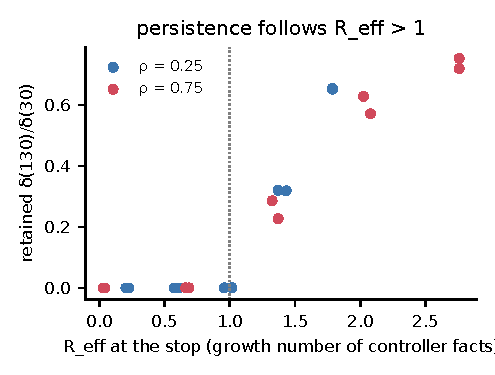
\includegraphics[width=0.44\linewidth]{fig4_threshold.pdf}
\caption{\textbf{Retained influence against $\mathcal R_C$} in the mean-field model.}
\label{fig:thr}
\end{figure}

\paragraph{Where the mean field fails.}
\begin{itemize}
\item Its controller effect is 3--10 times smaller than the simulator's ($g\approx0.07$--$0.09$).
\item It reaches its post-stop plateau within 5--9 time units, with no slow fading.
\end{itemize}
Both failures are finite-size effects.

% ======================================================================================================================
\section{Finite size: copies per fact}
\label{sec:finite}
\paragraph{The finite model.} The same rules, played out with discrete agents. No Bayesian engine is involved:
\begin{itemize}
\item $N=24$ agents, each with a binary memory over $F_A=16$ native and $F_C=4$ controller facts. Agent $i$ starts with
  native fact $i \bmod 16$.
\item Time steps of $dt=0.05$:
  \begin{itemize}
  \item each held fact is forgotten with probability $1-\rho^{dt}$;
  \item each agent acts with probability $dt$.
  \end{itemize}
\item An acting agent:
  \begin{itemize}
  \item reads $q$ posts with replacement from the 48 newest posts that are not its own;
  \item votes $A2$ with probability $\sigma(h_0+\beta_C n_C-\beta_A n_A)$ on its own counts;
  \item posts one item with the weights of Section~\ref{sec:repost}, gated by its own sampled vote.
  \end{itemize}
\item The controller posts a uniformly chosen controller fact with probability $\lambda_0\,dt$ per step until $T$.
\end{itemize}
A fact is \emph{lost} when it is absent from all memories and all readable windows. Since there is no reintroduction,
that state is absorbing. The model measures $\Delta_v$, from 400 paired episodes per point.

\paragraph{The system size is copies per fact.} Table~\ref{tab:copies} gives the stored simulator values. There are
only 1.5--12 copies per fact, so each fact's copy number is a small-population birth--death process with an absorbing
state at zero. Moreover, at the mean-field state each native fact is close to its own threshold,
$\mathcal R_f\approx0.8$--$1.1$: a near-critical branching process.
\begin{table}[h]
\centering\small
\caption{\textbf{Copies per fact in the simulator} (stored runs, $q=6$, $t=30$, controlled arm).}
\label{tab:copies}
\begin{tabular}{@{}lrrrr@{}}\toprule
cell & native: on board / holders & controller: on board / holders\\\midrule
task003 no-proof $\rho=0.25$ & 9.0 / 7.7 & 7.6 / 7.2\\
task003 symmetric $\rho=0.75$ & 4.4 / 12.2 & 4.0 / 11.0\\
OP no-proof $\rho=0.25$ & 6.2 / 6.5 & 5.6 / 6.1\\
OP no-proof $\rho=0.75$ & 4.3 / 11.4 & 3.6 / 10.7\\\bottomrule
\end{tabular}
\end{table}

\paragraph{Exact lineage results (ChatGPT agent).}
\begin{itemize}
\item \textbf{Critical birth--death lineage} (birth and death rate both 1), started from $c$ copies:
  \begin{equation}
  \Pr[\text{extinct by }t]=\Big(\frac{t}{1+t}\Big)^{c},\qquad \E[n(t)]=c .
  \end{equation}
  The mean is conserved while lineages die. With $F$ facts sharing a fixed total of $Fc$ copies, the expected number of
  surviving facts is $F[1-(t/(1+t))^c]$, so spreading the same total over more facts loses a larger fraction of them.
\item \textbf{Bounded neutral copying} (a Moran process with $K$ slots) gives the same lesson, exactly:
  \begin{equation}
  \E[\text{surviving facts}]=F\,[1-P_t(c,0)],
  \end{equation}
  where $P_t=e^{tQ}$ is the transition matrix of one fact's copy number.
\end{itemize}
Mean copy numbers, which are all a mean field tracks, cannot determine surviving diversity.

\begin{result}[asymmetric extinction]
With P0 parameters unchanged and nothing fitted:
\begin{itemize}
\item \textbf{Diversity collapse.} At $t=30$, 1.6 of 16 native facts still circulate at $\rho=0.1$, and 11.5 at
  $\rho=0.9$. All 4 controller facts survive.
\item \textbf{Effect size.} The controller effect rises from 0.07--0.09 (mean field) to 0.31--0.41, a magnitude
  comparable to selected simulator conditions. The model's reading, posting and controller policies differ from the
  simulator's, so this is not a matched validation.
\item \textbf{The reversal remains,} with the crossover at $\rho\approx0.5$--$0.6$.
\item \textbf{Lasting damage.} Removing the controller's facts at $T$ leaves a residual effect of $+0.036$.
\item \textbf{Approach to the mean field.} Replicating the swarm $R=1,2,4$ times, with the facts unchanged, gives
  $G=0.31,0.21,0.13$.
\end{itemize}
\end{result}

\paragraph{Mechanism.} The swarm's evidence is spread over many facts with few copies each, and these die out. The
controller recycles a few facts with many copies, and these survive. Extinction removes the swarm's protection but not
the controller's push. In a control spreading the same total controller evidence over 16 facts, the amplification over
the mean field fell from $4.2\times$ to $2.4\times$.

\paragraph{The number of surviving facts.} Two analytic approximations from mean-field rates bracket it at every memory
computed:
\begin{itemize}
\item independent two-type branching (holder and board) underestimates it: 0.12--9.4 surviving facts;
\item neutral drift at conserved total overestimates it: 3.6--16;
\item the finite model lies between: 3.0--12.0.
\end{itemize}
This is an observed bracket, not a proven bound.

\paragraph{Gating makes persistence fade.}
\begin{itemize}
\item With neutral reposting, the finite model retains 0.91--0.99 of its effect after 100 time units.
\item With vote-gated reposting ($\varepsilon=0.5$), it retains 0.55 and 0.30 and is still falling (Fig.~\ref{fig:gate}).
\end{itemize}
Controller lineages lose their reposters and go extinct one at a time. In this model, fading happens through loss of
exposure.
\begin{figure}[h]
\centering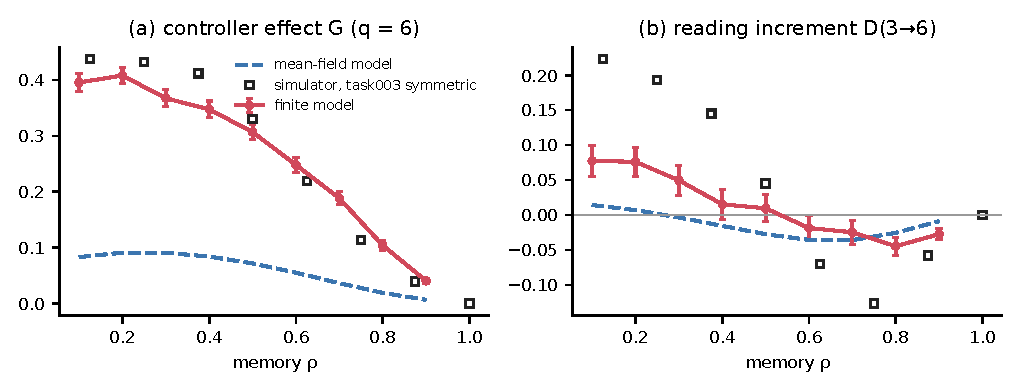
\includegraphics[width=0.95\linewidth]{fig5_finite_reversal.pdf}
\caption{\textbf{Finite against mean-field model.} The simulator (task003 symmetric) is shown for reference only.}
\label{fig:finite}
\end{figure}
\begin{figure}[h]
\centering
\begin{minipage}{0.42\linewidth}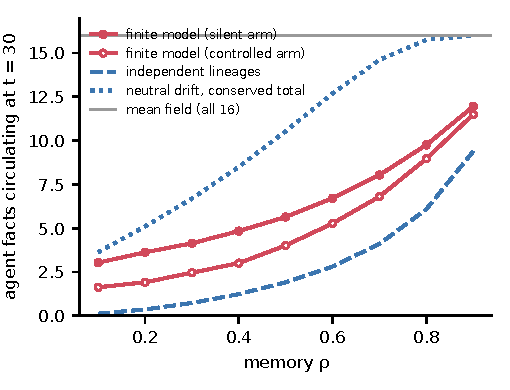
\includegraphics[width=\linewidth]{fig6_diversity.pdf}\end{minipage}\hfill
\begin{minipage}{0.56\linewidth}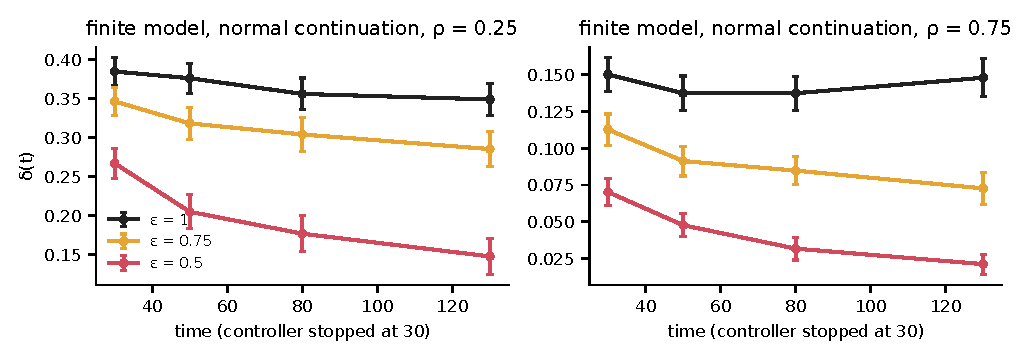
\includegraphics[width=\linewidth]{fig9_gating.pdf}\end{minipage}
\caption{\textbf{Left:} native facts circulating at $t=30$ in the finite model, with the two analytic approximations.
\textbf{Right:} vote gating in the finite model turns flat persistence into slow fading.}
\label{fig:gate}
\end{figure}

% ======================================================================================================================
\section{Heterogeneity of the evidence response}
\label{sec:response}
Equation~\eqref{eq:bayes} gives the exact persuasion of adding a fact to a memory:
\begin{equation}
\Delta P(M,f)=\sigma\big(x(M)+\theta_f(M)\big)-\sigma\big(x(M)\big).
\end{equation}
Approximation~\ref{ap:response} replaces $\theta_f(M)$ by $+\beta_C$. Measurements on stored memories test this.
\begin{itemize}
\item \textbf{Pre-registered.} The tested count and selected-motif parametrisations do not predict $\Delta P$ on held-out
  episodes ($R^2\approx0$). This shows that those parametrisations fail, not that every count or combination model
  must.
\item \textbf{Post-hoc.} The identity of the controller fact explains $R^2=0.38$--$0.78$.
\item \textbf{ChatGPT's extension,} prompted by that result. With flexible per-fact baselines and native-identity
  controls, pair and triple terms reduce held-out error by a further 9--26\% in all four setups.
\item \textbf{Sign changes.} The same controller fact can push towards or away from $A2$ in memories with equal counts.
  This is a sign change of $\theta_f(M)$ with context, which no fixed per-fact strength can produce.
\end{itemize}

\paragraph{Population susceptibility.} The linear response of the population to the controller facts it actually
encounters is
\begin{equation}
\Sus(t)=\E_{M\sim\mu_t}\,\E_{f\sim w_t}\big[\Delta P(M,f)\big],
\end{equation}
with $\mu_t$ the distribution of memories and $w_t$ the mix of controller facts on the board. It is an
\emph{observable}, not a state variable with its own law. It falls by 36\% and 80\% in OP no-proof after the stop and
stays within $\pm5\%$ in task003 (Fig.~\ref{fig:sus}).
\begin{figure}[h]
\centering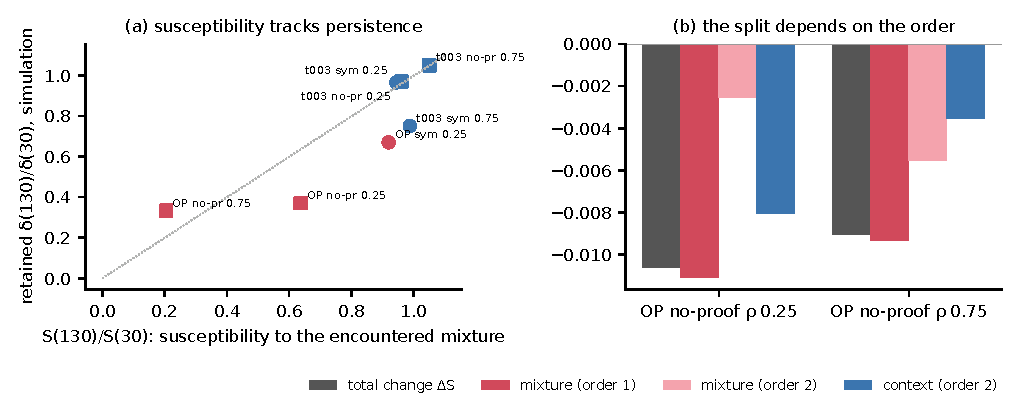
\includegraphics[width=0.95\linewidth]{fig10_susceptibility.pdf}
\caption{\textbf{(a)} Change in susceptibility against retained effect in the simulator. \textbf{(b)} Splitting the
change into ``mixture'' and ``context'' parts depends on the order of the split; the interaction is large.}
\label{fig:sus}
\end{figure}

% ======================================================================================================================
\section{Fading: selection among circulating controller facts}
\label{sec:fading}
\paragraph{What the simulator shows.} In OP no-proof:
\begin{itemize}
\item the controller's board share $b_C$ is flat after the stop ($-1\%$, $+5\%$);
\item the belief gap $\Delta_p$ falls 59\% and 89\% ($\rho=0.25$, $0.75$), and $\Sus$ falls 36\% and 80\%.
\end{itemize}
So in OP the effect fades \emph{at constant exposure}, unlike the finite model's gated fading. Two further measurements:
\begin{itemize}
\item \textbf{A frozen-strength probe.} Pairing the stop-time distribution of log-odds strengths with the later
  operating points does not reproduce the fall. This supports a change in conditional response, though it does not
  exclude every account based on correlations between operating point and context.
\item \textbf{The direction of the push.} In task003, 86--99\% of encountered (agent, controller fact) pairs push toward
  $A2$; in OP, only 53--70\%.
\end{itemize}

\paragraph{Coherence.} Let $c_f$ be the share of contexts, in a stated reference distribution (silent-arm memories at
$t=30$), in which adding $f$ raises $P(A2)$. It measures sign consistency and ignores magnitudes and zero-effect
contexts.

\paragraph{Selection model.} The fact-flow model is extended by tracking each controller fact separately. With
probability $c_f$, a fact moves its holder's log-odds by $+\beta_C$, and otherwise by $-\beta_C$, so
\begin{equation}
x=h_0-\beta_A M_A+\beta_C\sum_f m_f\,(2c_f-1).
\end{equation}
Support-based reposting gives the eligibility
\begin{equation}
g_f=\varepsilon+(1-\varepsilon)\Big[c_f\,\sigma(x+\beta_C)+(1-c_f)\big(1-\sigma(x-\beta_C)\big)\Big].\label{eq:gf}
\end{equation}

\paragraph{Derivation of Eq.~\eqref{eq:gf}.}
\begin{itemize}
\item With probability $c_f$ the fact pushes its holder toward $A2$. It then supports an $A2$ vote, cast with
  probability about $\sigma(x+\beta_C)$.
\item Otherwise it supports a non-$A2$ vote, cast with probability about $1-\sigma(x-\beta_C)$.
\end{itemize}
The holder-conditioned shift $\pm\beta_C$ is a crude closure. The exact own-fact shift is $\beta_f(1-m_f)$, plus
correlations.

\paragraph{The sign of selection.} Using $1-\sigma(y)=\sigma(-y)$,
\begin{equation}
\frac{\partial g_f}{\partial c_f}=(1-\varepsilon)\big[\sigma(x+\beta_C)-\sigma(\beta_C-x)\big],
\end{equation}
which has the sign of $x$. When most agents do not vote $A2$ ($x<0$), selection favours the \emph{least} coherent
facts: the majority recirculates controller facts in the contexts where they support its own answer. This is
frequency-dependent selection whose sign is set by the sign of the global field. If all coherences and magnitudes are
equal, the model has no coherence-based selection.

\paragraph{A Price equation for mean coherence.} Let $\bar c=\sum_f b_fc_f/b_C$ be the mean coherence on the board,
with $b_C=\sum_fb_f$. After the stop, $\dot b_f=\frac NW(S_f-b_f)$. Differentiating $\bar c$ gives exactly
\begin{equation}
\dot{\bar c}=\frac NW\,\frac{S_C}{b_C}\,\big(\bar c_{\rm new}-\bar c\big),\qquad
\bar c_{\rm new}=\frac{\sum_fS_fc_f}{\sum_fS_f},
\end{equation}
where $S_C$ is the probability that a new post carries a controller fact. Mean coherence relaxes toward the coherence of
what is being reposted. The equation matches the model's numerical derivative to four digits. It is a balance law, not
a closed equation:
\begin{itemize}
\item assuming $m_f\propto b_f$ gives a drift proportional to $\mathrm{Var}_b(c)$, which overestimates the drift 5--700
  times, because each fact's spread saturates;
\item the ChatGPT agent built two admissible states with equal $(b_C,\Sus,\bar c)$ but different coherence variance,
  whose $\Sus$ and $\bar c$ drifts differ. So no exact universal closure in these three variables exists on the
  model's state space. An approximate description on the trajectories actually reached is not excluded.
\end{itemize}

\paragraph{Pre-registered outcomes} (P0; ambivalent set $c=(0.9,0.7,0.5,0.3)$ against coherent set $c=0.97$):
\begin{itemize}
\item \textbf{Partly met.} $\bar c$ falls whenever reposting depends on the vote. The effect fades beyond exposure by
  0.15 at $\varepsilon=0.5$, but only 0.06--0.08 at $\varepsilon=0.75$ (threshold 0.1).
\item \textbf{Met.} The coherent set fades only as much as exposure.
\item \textbf{Met.} $\varepsilon=1$ gives no selection.
\item \textbf{Inconclusive.} The predicted flip under an $A2$ majority: the run did not create such a majority.
\item \textbf{Failed.} Coherence measured on the whole controller pool does not separate the tasks: task003 no-proof
  has the most spread-out pool.
\end{itemize}

\paragraph{Post-hoc evidence.}
\begin{itemize}
\item Weighting world coherence by the controlled arm's board shares separates the tasks: 0.77--0.89 in task003,
  unchanged after the stop, against 0.46--0.62 in OP, falling (Fig.~\ref{fig:sel}b). The controller circulates
  coherent facts when its pool has them.
\item Within episodes, surviving controller facts were \emph{more} persuasive than lost ones in task003, and
  \emph{less} persuasive in OP no-proof at $\rho=0.75$ ($-0.026\pm0.004$).
\item ChatGPT's pre-registered closure test: adding $\bar c$ to $(b_C,\Sus)$ improves forecasts materially only in OP
  no-proof $\rho=0.75$ (+5.5\% quadratic ridge; +3.8\% nearest neighbours, below the 5\% threshold).
\end{itemize}
The coherence of circulating facts was chosen post-hoc. It is neither an intrinsic world parameter nor a validated
cross-task mapping.
\begin{figure}[h]
\centering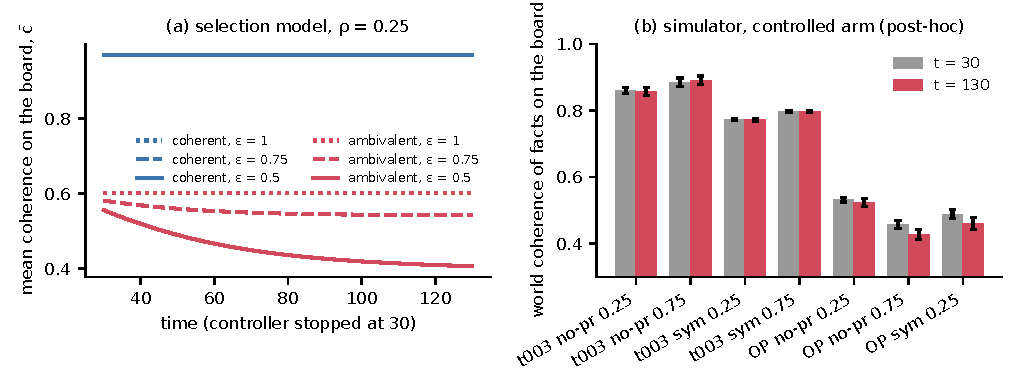
\includegraphics[width=0.95\linewidth]{fig_selection.pdf}
\caption{\textbf{(a)} Selection model: mean coherence on the board after the stop. \textbf{(b)} Simulator (post-hoc):
world coherence of the controller facts on the board at the stop and 100 time units later.}
\label{fig:sel}
\end{figure}

\paragraph{Two possible routes to fading.}
\begin{enumerate}
\item \textbf{Selection among circulating controller facts,} as above. It is supported where fading is strongest.
\item \textbf{Weakening response at fixed facts} as receiver contexts change. In OP no-proof at $\rho=0.25$, $\Sus$
  falls 36\% with no detectable identity selection and no closure gain from $\bar c$. This route has no explanatory
  law.
\end{enumerate}
These are possibilities within the framework, not a uniquely identified causal partition of individual cells.

% ======================================================================================================================
\section{An alternative closure: exact co-retention (ChatGPT agent)}
\label{sec:gpt}
The ChatGPT agent built an independent model around a different response. A repeated controller claim $C$ competes with
information whose meaning requires assembling $k$ interchangeable native facts. Single native facts are inert, and only
the full set corrects.

\paragraph{Co-retention.} Its central object is the exact co-retention moment $h_n$: the probability of holding a given
set of $n$ native facts. Because a single read can bring several facts at once, held facts are correlated even though
each is forgotten independently. Exactly,
\begin{equation}
\dot h_n=-n\gamma\,h_n+\sum_{j=1}^{n}P_n(j)\,\big(h_{n-j}-h_n\big),\qquad h_0=1,
\end{equation}
where $P_n(j)$ is the probability that one read brings exactly $j$ of the $n$ facts. Products of single-fact
probabilities systematically underestimate $h_n$.

\paragraph{Reduction.} With memory fast compared with the board, the moments become stationary functions of the
controller's board share $b$. Only two variables then evolve:
\begin{equation}
\dot b=\nu\{w_C(b)-b[w_A(b)+w_C(b)]\}+J(t)(1-b),\qquad \dot v=\Phi(b)-v,
\end{equation}
with:
\begin{itemize}
\item the response $\Phi=p_0-\beta\tilde h_k+\alpha(\tilde j_0-\eta\tilde j_k)$, where tildes denote memory just after
  reading and $j_n$ the probability of holding $C$ together with a given set of $n$ native facts;
\item $v$ the mean last vote, $\nu=N/W$, and $J(t)$ the controller's posting rate.
\end{itemize}

\paragraph{Results.}
\begin{itemize}
\item The reversal appears at $k=6$ and fails at $k=2$ and $3$. So a full-proof conjunction cannot be read as the proof
  size of the task, and it is not our default explanation.
\item Persistence appears as invasion of the controller-free state, with growth numbers 1.27 and 1.59 and no
  bistability. This is a threshold of the same kind as Eq.~\eqref{eq:R}, derived independently.
\end{itemize}

% ======================================================================================================================
\section{The common framework and its status}
\label{sec:status}
The two agents agreed on the following, in a signed statement on the shared blackboard.
\begin{enumerate}
\item \textbf{Circulation.} Facts are copied between memories and readable windows and are forgotten. The local
  invasion threshold is $\mathcal R_C>1$.
\item \textbf{Evidence response.} The next vote responds to the net log-odds displacement through a sensitivity that
  depends on the operating point. The reading reversal is the competition of Eq.~\eqref{eq:rev}.
\item \textbf{Irreversible loss of diversity.} In a finite swarm, the system size is copies per fact. Asymmetric
  extinction sets the size of the effect and the lasting damage.
\end{enumerate}
The response depends on context, but there is no agreed compact representation of that dependence. Fading has two
possible routes (Section~\ref{sec:fading}).

\paragraph{Not explained.}
\begin{itemize}
\item The size of $D$: the finite model's is 2--3 times too small.
\item The crossover position $\rho^*(q)$.
\item The order of the two no-proof setups.
\item The scaling with $K$ copies of the project at $K=4$.
\item Route 2 of fading.
\item The size of the fading at realistic reposting eligibility.
\item The predicted flip of selection under an $A2$ majority.
\item Whether rare proof holders matter through their later posts.
\end{itemize}

\paragraph{Pre-registered and post-hoc.}
\begin{itemize}
\item \textbf{Pre-registered,} with failures reported: the reversal and threshold of the fact-flow model, the finite-model
  expectations, the $\beta_A$ ordering, the count/motif test, the susceptibility probe, the fading-chain predictions,
  and the selection-model predictions.
\item \textbf{Post-hoc:} the identity result, the survival-by-persuasion comparison, and the coherence of circulating
  facts.
\end{itemize}
An out-of-sample test of the coherence parameter, on a setup not used to find it, is left as future work.

\paragraph{Lessons for a physicist.} The phenomena are not properties of the inference engine. They emerge from four
generic ingredients:
\begin{itemize}
\item a two-stage copying process with a reproduction-number threshold;
\item a bounded (logistic) response whose susceptibility peaks at a tipping point;
\item absorbing extinction at small copy numbers;
\item frequency-dependent selection whose sign is set by the global field.
\end{itemize}
The exact Bayesian structure enters only through effective parameters ($\beta_A$, coherence) and through a context
dependence of the response that no exchangeable closure captures.

\paragraph{Sources.}
\begin{itemize}
\item Models: \nolinkurl{analysis/theory_claude/phenomenological_fact_flow/} (\nolinkurl{fact_flow.py},
  \nolinkurl{finite_model.py}) and \nolinkurl{analysis/theory_claude/fading_chain/selection_model.py}.
\item Measurements: \nolinkurl{discriminating_test/}, \nolinkurl{mixture_probe/}, \nolinkurl{fading_chain/}.
\item ChatGPT's work: \nolinkurl{analysis/theory_chatgpt/}.
\item The shared statement: \nolinkurl{analysis/theory_blackboard/}\\ \nolinkurl{2026-10-28_claude_18_common_theory_REVISED.md}.
\end{itemize}

\end{document}
